% Exploration note for PB3D issue #4, in the layout of T. Weyens, "Expressions
% for perturbed vacuum potential energy for 3D linear MHD stability" (2019).
% Build: latexmk -pdf report.tex   (figures: scripts/vacuum_wave/figures.py)
\documentclass[%
 aip,
 rsi,%
 amsmath,amssymb,
 reprint,%
]{revtex4-1}

\usepackage[pdfusetitle,colorlinks,
 filecolor={[rgb]{0,0,1}},urlcolor={[rgb]{0,0,1}},
 citecolor={[rgb]{0,0,.4}},linkcolor={[rgb]{0,0,.4}},
 plainpages=false,pdfpagelabels]{hyperref}
\usepackage{graphicx}% Include figure files
\usepackage{amsmath}
\usepackage{bm}% bold math
\usepackage{esint} % various fancy integral symbols

\begin{document}

% USE BOLDFACE FOR (UNIT) VECTORS AND MATRICES
\let\oldhat\hat
\renewcommand{\vec}[1]{\bm{#1}}
\renewcommand{\hat}[1]{\oldhat{\bm{#1}}}
\newcommand{\mtx}[1]{\underline{\mathrm{#1}}}

% USE UPRIGHT DIFFERENTIAL d
\renewcommand{\d}[1]{\ensuremath{\operatorname{d}\!{#1}}}

% JACOBIAN
\newcommand{\J}{\mathcal{J}}

% PRINCIPAL VALUE INTEGRAL
\newcommand{\pvint}{\fint}

% LET TWO WIDE FIGURES SHARE THE TOP OF A PAGE; NO STRETCHED COLUMNS
\renewcommand{\dbltopfraction}{0.9}
\renewcommand{\topfraction}{0.9}
\raggedbottom

\title[Exploration note, PB3D issue \#4 --- Keeping integrals instead of points in the field-line vacuum]{Keeping integrals instead of points: a wave-amplitude form of the field-line vacuum of PB3D}

\author{Claude Opus 5.5 and Claude Fable 5.1}
 \affiliation{Anthropic. Written for Toon Weyens as an exploration note for PB3D issue \#4 on 3 November 2026 and checked and revised on 4 November; nothing in it is decided or required.}

\date{4 November 2026}

\begin{abstract}
In PB3D, a Richardson level doubles the number of points along each field line.
The plasma integrals keep only their value from the previous level, but the field-line vacuum solves for the potential at every boundary point, with two dense $N\times N$ matrices that grow fourfold with every level.
This note shows that the same boundary equation, written for the amplitudes of a few dozen waves $e^{\imath(n\varphi - m\theta)}$ instead of the values at the $N$ points, keeps only sums over pairs of points.
A Richardson level then reuses one quarter of the previous level's sums and adds the pairs that contain a new point, and no $N\times N$ matrix is ever stored.
A Python prototype on a circular torus, with exact toroidal harmonics as the test, meets the four criteria that were fixed before the runs: the carried-over sums equal the sums computed from scratch to $9\times10^{-16}$; with 34 waves for a window of 10 modes the vacuum energy equals that of the point-value solve on the same rows to $4\times10^{-6}$; and 51\,264 boundary points run in 1.9~GB in total, of which the method itself needs about 1.2~GB, against 21~GB for one $N\times N$ matrix.
With single waves as data, as the plasma modes of PB3D are, the potential stays on the wave of the data, and three or four sidebands on each side of the mode window would do.
The near-field rule of PB3D, stellarator geometry and the Fortran implementation are not tested.
\end{abstract}

\maketitle

\section{Introduction}
PB3D \cite{Weyens2017PB3D} uses Richardson extrapolation in the number of points along the magnetic field lines.
Each level replaces $n_\text{par}$ points per field line by $2n_\text{par}-1$: the old points stay, and a new point is placed halfway between each pair of neighbours.
In the plasma, every field-line integral is a sum of independent contributions of the points.
The routine \texttt{calc\_magn\_ints} therefore keeps only the value of each integral: it halves it, because the step size halves, and adds the contributions of the new points.
Section VI of Ref.~\onlinecite{Weyens2019vacuum} remarks that the vacuum cannot do the same: ``for the boundary method all the data points are needed''.

The reason is that the vacuum potential at one boundary point depends on the potential at all the others.
With the potential at the $N$ boundary points as unknowns, the boundary element method needs two dense $N\times N$ matrices, $\mtx{G}$ and $\mtx{H}$, and a dense solve.
Doubling the parallel points doubles $N$ and quadruples the matrices.
With 128 field lines and 400 points per line, $N = 51\,200$; one such matrix of double-precision numbers takes 21~GB, and the PB3D run at that size was given 220~GB.

The remark in Ref.~\onlinecite{Weyens2019vacuum} holds as long as the unknowns are point values.
This note changes the unknowns to the amplitudes of a set of waves on the boundary and shows that the vacuum can then also keep only sums from one level to the next.
Section~\ref{sec:points} recalls the point-value form, section~\ref{sec:waves} derives the wave form, section~\ref{sec:richardson} gives the Richardson step, section~\ref{sec:prototype} reports a prototype on a circular torus and section~\ref{sec:open} lists what it does not test.

\section{The point-value form}\label{sec:points}
Let $\vec{n}$ be the unit normal on the plasma boundary $S$ that points out of the plasma, into the vacuum, and $q = \partial\Phi/\partial n$ the normal derivative of the vacuum potential $\Phi$, which the plasma displacement fixes.
For a potential that is harmonic outside $S$ and decays at infinity, Green's second identity gives, for every point $\vec{x}$ on a smooth part of $S$,
\begin{equation}
2\pi\,\Phi(\vec{x}) - \pvint_S \Phi(\vec{y})\,K(\vec{x},\vec{y})\,\d{S_y} = -\oint_S G(\vec{x},\vec{y})\,q(\vec{y})\,\d{S_y} \ ,
\label{eq:bie}
\end{equation}
with
\begin{equation}
G(\vec{x},\vec{y}) = \frac{1}{\left|\vec{x}-\vec{y}\right|} \ , \qquad
K(\vec{x},\vec{y}) = \frac{(\vec{x}-\vec{y})\cdot\vec{n}_y}{\left|\vec{x}-\vec{y}\right|^3} \ .
\end{equation}
This is the exterior form of the boundary equation of Ref.~\onlinecite{Weyens2019vacuum}, written with the normal that points out of the plasma.

The boundary is sampled at the points of the field-line grid of PB3D (Fig.~\ref{fig:grid}): $n_\alpha$ field lines, each followed over one poloidal turn with $n_\text{par}$ points, $N = n_\alpha n_\text{par}$ points in total.
A surface integral becomes a sum with weights $w_j = \Delta\alpha\,\Delta\theta_j\,\J_S(\vec{x}_j)$, where $\J_S$ is the surface Jacobian of the coordinates $(\alpha,\theta)$ and $\Delta\theta_j$ is the step along the line, halved at the two ends of each line (trapezoidal rule).

\begin{figure}[t]
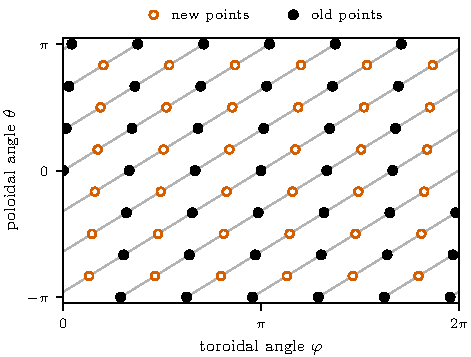
\includegraphics[width=\columnwidth]{fig_grid.pdf}
\caption{Field-line grid on the torus surface, unrolled in the toroidal angle $\varphi$ and the poloidal angle $\theta$: 6 field lines $\varphi = \alpha + q\theta$ with $q = 1.043$. A Richardson level keeps the old points (black) and adds one new point (open) between each pair of neighbours along each line. The prototype uses 16 to 128 lines and 51 to 801 points per line.}
\label{fig:grid}
\end{figure}

PB3D's field-line vacuum (\texttt{vac\%style} 1) asks Eq.~\eqref{eq:bie} to hold exactly at each of the $N$ points (collocation):
\begin{equation}
\sum_{j} H_{ij}\,\Phi_j = -\sum_{j} G_{ij}\,q_j \ , \qquad i = 1,\ldots,N \ ,
\label{eq:collocation}
\end{equation}
with, for $j \neq i$,
\begin{equation}
H_{ij} = -w_j\,K(\vec{x}_i,\vec{x}_j) \ , \qquad G_{ij} = w_j\,G(\vec{x}_i,\vec{x}_j) \ .
\label{eq:offdiag}
\end{equation}
The diagonal elements stand for the integrals over the cell around $\vec{x}_i$, where the kernels are singular.
As in \texttt{calc\_GH\_1}, they follow from potentials that are harmonic inside the plasma and known exactly.
The constant $\Phi = 1$ has $q = 0$; inside, Eq.~\eqref{eq:bie} reads $-2\pi\Phi - \pvint\Phi K\,\d{S} = -\oint G q\,\d{S}$, so the principal-value integral of $K$ equals $-2\pi$, and the self term of $K$ is $c_i = -2\pi - S_i$ with $S_i = \sum_{j\neq i} w_j K(\vec{x}_i,\vec{x}_j)$.
In the exterior equation~\eqref{eq:bie} this gives
\begin{equation}
H_{ii} = 2\pi - c_i = 4\pi + S_i \ .
\end{equation}
The linear potentials $x$, $y$ and $z$ have $q = n_x$, $n_y$, $n_z$ and give the self term $G_{ii}$ of $G$ in the same way, as a least-squares fit over the three potentials.

Every row of Eq.~\eqref{eq:collocation} involves every point, so the matrices have $N^2$ entries.
Fig.~\ref{fig:matrices}(a) shows $|H_{ij}|$ on a small grid: the matrix is full, with the largest entries where $\vec{x}_i$ and $\vec{x}_j$ are close on the surface.

\section{The wave form}\label{sec:waves}
\subsection{What the potential looks like}
For a perturbation with toroidal mode number $n$, the boundary data $q$ and the potential $\Phi$ vary as $e^{\imath n \varphi}$ times a function of $\theta$, on an axisymmetric boundary.
In a straight cylinder, data with one poloidal mode number $m$ give a potential with that same $m$ only.
On a torus a potential also contains other poloidal mode numbers, and how many depends on the angle in which the waves are written.

Fig.~\ref{fig:spectrum} shows this for the exact exterior harmonics used in section~\ref{sec:prototype}, on a torus of aspect ratio 3, with waves in the geometric poloidal angle $\theta$.
Each harmonic is a single wave $e^{-\imath m u}$ in the angle $u$ of toroidal coordinates.
On the torus surface the two angles are related by $\tan\theta = \sinh\eta_0 \sin u/(\cosh\eta_0\cos u - 1)$ with $\cosh\eta_0 = R_0/a = 3$, so $\d{u}/\d{\theta}$ runs from $\tanh(\eta_0/2) = 0.71$ on the outboard side to $\coth(\eta_0/2) = 1.41$ on the inboard side, and $u - \theta$ reaches 0.345~rad at $\theta = \pm1.74$.
The upper panel shows the result for $m = 11$: the potential oscillates more slowly than $\cos 11\theta$ on the outboard side and faster on the inboard side, where its amplitude $\sqrt{\cosh\eta_0 - \cos u}$ is also larger, by $\sqrt{2}$.
In $\theta$ the local poloidal wavenumber of a harmonic, $m\,\d{u}/\d{\theta}$, runs from $0.71m$ to $1.41m$, so the harmonic needs waves over at least that range, plus a margin for the variation of its amplitude.
The lower panel gives the amplitudes of the waves $e^{\imath(n\varphi-m\theta)}$ in the three harmonics.
They are spread over a band that widens with $m$: amplitudes above 0.1 of the largest for $m = 3$ to 10 in the harmonic $m = 6$, 7 to 18 in $m = 11$ and 9 to 24 in $m = 15$, and above $10^{-3}$ for $m = 2$ to 14, 4 to 22 and 7 to 29.
Outside the band the amplitudes fall steeply.
The 34 waves of the prototype, $m = -6$ to 27, cover the bands of $m = 6$ and 11 to below $10^{-5}$ and that of $m = 15$ to $8\times10^{-3}$, its amplitude at $m = 27$.

\begin{figure}[t]
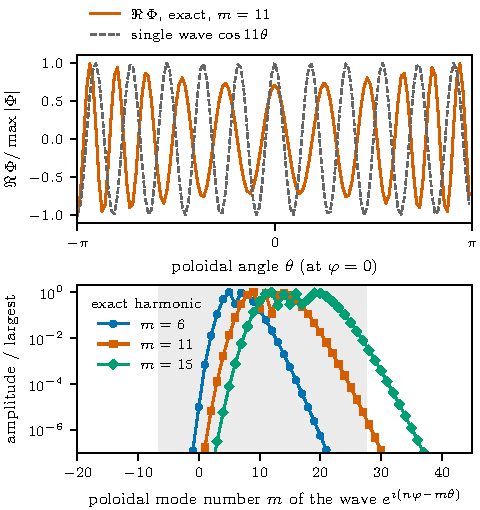
\includegraphics[width=\columnwidth]{fig_spectrum.pdf}
\caption{The potential of the exact exterior harmonics on the torus ($R_0 = 3$, $a = 1$, $n = 10$), at $\varphi = 0$. (a) Real part of the $m = 11$ harmonic, normalised, against the single wave $\cos 11\theta$. (b) Amplitudes of the waves $e^{\imath(n\varphi - m\theta)}$ in the harmonics $m = 6$, 11 and 15, each normalised to its largest; the waves use the geometric angle $\theta$, in which each harmonic is spread over many $m$. The grey band is the set of 34 waves used in the prototype, $m = -6$ to 27.}
\label{fig:spectrum}
\end{figure}

\subsection{Unknowns and equations}
Two changes turn Eq.~\eqref{eq:collocation} into a small system.
First, the potential is written as a sum of $M'$ waves,
\begin{equation}
\Phi(\vec{x}) = \sum_{k=1}^{M'} a_k\,e_k(\vec{x}) \ , \qquad e_k(\vec{x}) = e^{\imath\left(n\varphi - m_k\theta\right)} \ ,
\label{eq:waves}
\end{equation}
so that the unknowns are the $M'$ amplitudes $a_k$ instead of the $N$ values $\Phi_j$.
Second, Eq.~\eqref{eq:collocation} is no longer required at every point.
Instead, the error of Eq.~\eqref{eq:collocation} at each point $i$ is multiplied by $w_i\,\bar{e}_l(\vec{x}_i)$ and summed over all points; this sum is set to zero for each of the $M'$ waves $l$.
In words: the error may remain, but it must not contain any of the $M'$ waves.
This is the Galerkin method \cite{Sauter2011BEM}.
A Fourier representation of the vacuum potential is also what NESTOR \cite{Merkel1986} and the free-boundary version of CAS3D \cite{Merkel1996} use, on a regular $(\theta,\varphi)$ grid; here it is combined with the field-line points of PB3D and with the Richardson step.
It gives $M'$ equations for the $M'$ amplitudes,
\begin{equation}
\sum_{k=1}^{M'} A_{lk}\,a_k = b_l \ , \qquad l = 1,\ldots,M' \ ,
\label{eq:galerkin}
\end{equation}
with
\begin{align}
A_{lk} &= \sum_{i=1}^{N}\sum_{j=1}^{N} w_i\,\bar{e}_l(\vec{x}_i)\,H_{ij}\,e_k(\vec{x}_j) \ , \label{eq:A}\\
b_l &= -\sum_{i=1}^{N}\sum_{j=1}^{N} w_i\,\bar{e}_l(\vec{x}_i)\,G_{ij}\,q_j \ . \label{eq:b}
\end{align}
In the notation of section V of Ref.~\onlinecite{Weyens2019vacuum}, with $\mtx{E}'$ the $N\times M'$ matrix of the waves at the points and $\mtx{I}$ the diagonal matrix of the weights,
\begin{equation}
\mtx{A} = \mtx{E}'^\dagger\,\mtx{I}\,\mtx{H}\,\mtx{E}' \ , \qquad \vec{b} = -\mtx{E}'^\dagger\,\mtx{I}\,\mtx{G}\,\vec{q} \ .
\end{equation}
$\mtx{E}'$ has the same form as $\mtx{E}$ in Eq.~(106) of that reference, with more columns, because the potential needs the neighbouring $m$ of each mode of the plasma window.
The vacuum energy follows from the amplitudes as
\begin{equation}
-\oint_S \bar{q}\,\Phi\,\d{S} \approx -\sum_{i} w_i\,\bar{q}_i \sum_k a_k\,e_k(\vec{x}_i) \ ,
\end{equation}
which is the quantity that PB3D needs in its edge block.

\subsection{Why no $N\times N$ matrix is needed}
Each entry of Eqs.~\eqref{eq:A} and~\eqref{eq:b} is a double sum over pairs of points $(i,j)$: the point $i$ where the equation is tested and the point $j$ whose source acts there.
The double sums can be built one block of rows at a time.
For a block of a few hundred points $i$, the kernel values $H_{ij}$ and $G_{ij}$ are computed for all $j$, multiplied by the waves and the data at $\vec{x}_j$, and then by $w_i\,\bar{e}_l(\vec{x}_i)$, and added to $\mtx{A}$ and $\vec{b}$.
The block is then discarded.
What stays in memory is $\mtx{A}$ ($M'\times M'$), $\vec{b}$, the waves at the points ($N\times M'$) and one block of kernel values.
The self terms of section~\ref{sec:points} need only three sums per point, $S_i$, $\sum_{j\neq i} w_j K_{ij}\,\vec{x}_j$ and $\sum_{j\neq i} w_j G_{ij}\,\vec{n}_j$, which are accumulated with the same blocks.

Fig.~\ref{fig:matrices}(b) shows $|A_{lk}|$ for 34 waves.
Its size does not depend on $N$, and it is nearly tridiagonal: the median ratio to the diagonal is $0.17$ for the first neighbours, $3\times10^{-4}$ for the second and $4\times10^{-5}$ for the third.
Most of $\mtx{A}$ is the term $2\pi\Phi$ of Eq.~\eqref{eq:bie}, which gives $2\pi M_{lk}$ with $M_{lk} = \sum_i w_i\,\bar{e}_l(\vec{x}_i)\,e_k(\vec{x}_i)$ the mass matrix of the waves.
On the torus $\d{S}$ contains the factor $R_0 + a\cos\theta = R_0 + \tfrac{a}{2}(e^{\imath\theta} + e^{-\imath\theta})$, so $\mtx{M}$ couples each wave to its two neighbours only, with the ratio $a/(2R_0) = 1/6$; the discrete $\mtx{M}$ reproduces this to $10^{-15}$.
The double-layer part $\mtx{A} - 2\pi\mtx{M}$ is 0.5\,\% of the diagonal of $\mtx{A}$ and 0.6\,\% at the first neighbours, and it is all of the second and third neighbours.
So the operator couples each wave mainly to its two neighbours, and the wide bands of Fig.~\ref{fig:spectrum} come from the data of the test harmonics, which are as spread as the potentials.
Section~\ref{sec:prototype} shows what happens with single waves as data, as the plasma modes of PB3D are.

\begin{figure*}[t]
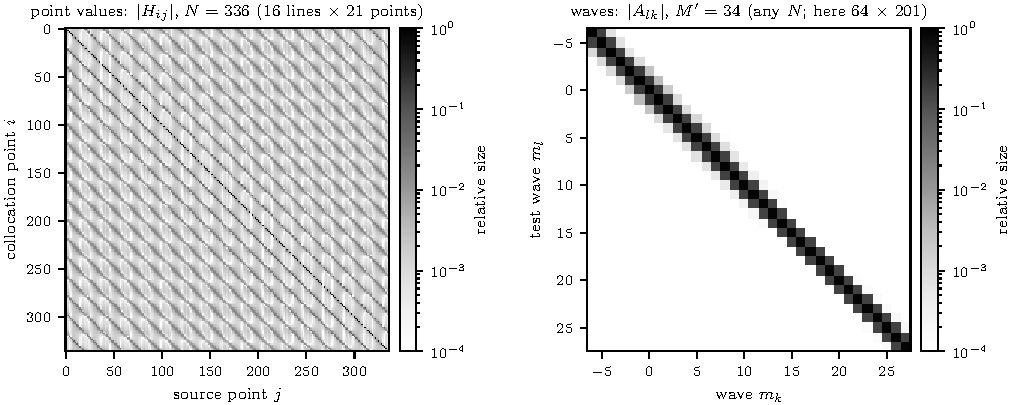
\includegraphics[width=\textwidth]{fig_matrices.pdf}
\caption{What each method solves with. (a) $|H_{ij}|$ of the point-value form on a grid of 16 lines $\times$ 21 points, normalised to its largest entry: a full $N\times N$ matrix, which at 51\,200 points has $2.6\times10^{9}$ entries. (b) $|A_{lk}|$ of the wave form, Eq.~\eqref{eq:A}, for the 34 waves $m = -6,\ldots,27$, computed on 64 lines $\times$ 201 points: $34\times34$ entries for any number of points.}
\label{fig:matrices}
\end{figure*}

\section{The Richardson step}\label{sec:richardson}
When a Richardson level halves the step along the lines, every old point keeps its position, its normal and its data, and its weight halves: $w_i \to w_i/2$ (also at the ends of the lines, where the weight is half a step).
The kernels $K(\vec{x}_i,\vec{x}_j)$ and $G(\vec{x}_i,\vec{x}_j)$ between two old points and the waves at old points do not change.
A term of Eq.~\eqref{eq:A} or~\eqref{eq:b} for a pair of old points carries the product $w_i w_j$ and is therefore multiplied by $\tfrac14$.

Split $\mtx{A}$ into the pairs with $i\neq j$ and the self terms,
\begin{align}
A^\text{pair}_{lk} &= -\sum_{i}\sum_{j\neq i} w_i w_j\,\bar{e}_l(\vec{x}_i)\,K(\vec{x}_i,\vec{x}_j)\,e_k(\vec{x}_j) \ , \\
A^\text{self}_{lk} &= \sum_{i} w_i\,\bar{e}_l(\vec{x}_i)\,\left(4\pi + S_i\right)e_k(\vec{x}_i) \ ,
\end{align}
and $\vec{b}$ in the same way.
From level $r$ to level $r+1$,
\begin{equation}
A^{\text{pair},(r+1)}_{lk} = \tfrac14\,A^{\text{pair},(r)}_{lk} + \sum_{\text{pairs with a new point}} (\ldots) \ ,
\label{eq:carry}
\end{equation}
where the last sum runs over the pairs (old $i$, new $j$), (new $i$, old $j$) and (new $i$, new $j$).
The per-point sums of the self terms carry one weight, so for an old point
\begin{equation}
S_i^{(r+1)} = \tfrac12\,S_i^{(r)} + \sum_{j\ \text{new}} w_j\,K(\vec{x}_i,\vec{x}_j) \ ,
\end{equation}
and likewise for the other two sums; a new point gets its full sums.
$\mtx{A}^\text{self}$ and the self part of $\vec{b}$ are then recomputed from the per-point sums, at a cost of $N M'^2$ operations.
Fig.~\ref{fig:carry} summarises the step.

\begin{figure}[t]
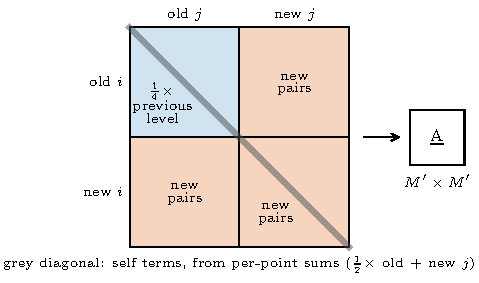
\includegraphics[width=\columnwidth]{fig_carry.pdf}
\caption{The pairs of points $(i,j)$ of one Richardson step, with the old points listed first. The pairs of two old points enter as one quarter of the previous level's sums; the other three blocks are computed. All of them are added straight into the $M'\times M'$ matrix $\mtx{A}$. The self terms on the diagonal come from per-point sums, which carry over as one half of the old sums plus the new columns.}
\label{fig:carry}
\end{figure}

This is the analogue of \texttt{calc\_magn\_ints} for a double integral.
The plasma keeps one number per integral and computes only the new points, half of the work of a level.
The wave form keeps $\mtx{A}$, $\vec{b}$ and three sums per point, and computes the pairs that contain a new point, three quarters of all pairs.
The memory grows twofold per level, with $N$, instead of fourfold; the work still grows with $N^2$.

Section VI of Ref.~\onlinecite{Weyens2019vacuum} lists three options for the vacuum under Richardson extrapolation: (A) store $\mtx{H}^{-1}\mtx{G}$ or $\mtx{H}$ and $\mtx{G}$ separately; (B) update the LU factors or the inverse of $\mtx{H}$ block by block; (C) store $\mtx{G}\mtx{E}\mtx{P}$ instead of $\mtx{G}$ and update it as an integral.
The wave form is a fourth option.
It is closest to (C), which applies the modes to $\mtx{G}$ from the right; the wave form applies them from both sides and to $\mtx{H}$ as well, so that no matrix of size $N$ remains.
Option (B) does not apply as written: by the argument above, the old-to-old block of the new $\mtx{H}$ has its off-diagonal entries halved and its diagonal recomputed from the new row sums, so it is not the previous level's $\mtx{H}$, and its LU factors cannot be reused.

\section{Prototype on a circular torus}\label{sec:prototype}
\subsection{Test case}
The prototype (\texttt{scripts/vacuum\_wave/prototype.py} on the branch \texttt{exp/vacuum-wave-prototype}) is written in Python.
The boundary is a circular torus with $R_0 = 3$ and $a = 1$, sampled on field lines $\varphi = \alpha + q\theta$ with $q = 1.04296875$; this value makes sure that no line end meets a line start for 16 to 128 lines.
The tests are exact exterior harmonics in toroidal coordinates $(\eta, u, \varphi)$ \cite{DLMF14},
\begin{equation}
\Phi_m = \sqrt{\cosh\eta - \cos u}\;P^{n}_{|m|-1/2}(\cosh\eta)\;e^{\imath(n\varphi - m u)} \ ,
\end{equation}
with $n = 10$ and $m = 6$, 11 and 15.
$P^n_{|m|-1/2}$ is evaluated from Laplace's integral, up to a constant factor.
A finite-difference Laplacian of $\Phi_m$ at three exterior points is below $2.2\times10^{-6}$ of its separate terms, the size of the difference error.
The normal derivative $q$ on the torus comes from fourth-order differences with step $10^{-3}a$, and the exact vacuum energy $-\oint\bar{q}\,\Phi\,\d{S}$ from a periodic $(\theta,\varphi)$ grid.

Both methods receive the exact $q$ at the points and solve for $\Phi$.
They use exactly the same rows of $\mtx{H}$ and $\mtx{G}$: the plain trapezoidal rule along and across the lines, with the self terms of section~\ref{sec:points}, and no near-field rule.
The comparison therefore isolates the change of unknowns.
The errors are the relative weighted $L_2$ error of $\Phi$ at the points and the relative error of the vacuum energy.
The waves are Eq.~\eqref{eq:waves} with $m$ from $6-k$ to $15+k$, i.e.\ $k$ sidebands on each side of the window of the three test harmonics.

The four criteria of Table~\ref{tab:criteria} were fixed before the runs.

\begin{table}[b]
\caption{Criteria fixed before the runs, and results.}
\label{tab:criteria}
\begin{ruledtabular}
\begin{tabular}{p{0.45\columnwidth}p{0.47\columnwidth}}
Criterion & Result \\
\hline
1. carried-over sums equal the sums from scratch to $10^{-12}$ & $4.7$ to $8.9\times10^{-16}$ at 101 to 801 points per line \\
2. wave form at most 1.5 times the point-value error on the same grid & energy errors equal to 3 digits; $\Phi$ errors 0.89 to 0.98 times those of the point values (64 $\times$ 201) \\
3. a small multiple of the mode window in waves & 34 waves for 10 modes \\
4. peak memory far below one $N\times N$ matrix & 1.9~GB for 51\,264 points, whole process; one $N\times N$ matrix: 21~GB \\
\end{tabular}
\end{ruledtabular}
\end{table}

\subsection{Number of waves}
Fig.~\ref{fig:accuracy}(a) gives the error of the vacuum energy against the number of sidebands $k$, on 64 lines $\times$ 201 points.
Without sidebands the errors are 6 to 55\,\%.
The harmonics $m = 6$ and 11 settle at $k = 6$ (22 waves), $m = 15$, which reaches furthest outside the window, at $k = 12$ (34 waves).
Beyond that the error no longer depends on the waves but on the quadrature of the kernels, and it equals that of the point-value form.
On the way the energy error can dip below its settled value ($m = 6$ at $k = 2$, $m = 11$ at $k = 1$, $m = 15$ at $k = 6$); these dips are cancellations in the energy, not better solutions, since the error of $\Phi$ there is 0.07, 0.12 and 0.18.

\begin{figure*}[t]
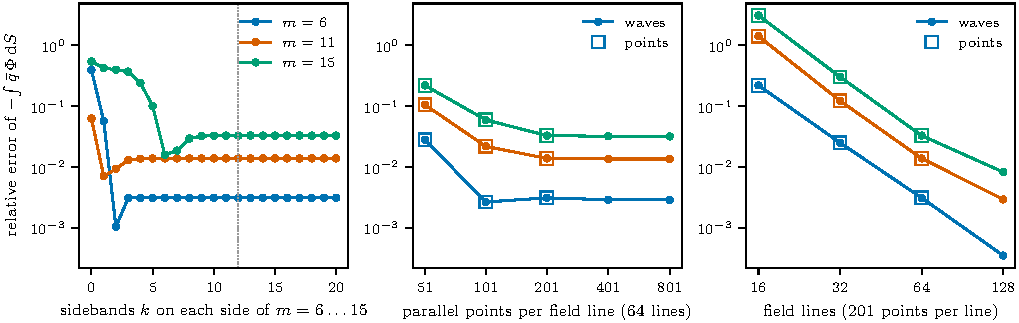
\includegraphics[width=\textwidth]{fig_accuracy.pdf}
\caption{Relative error of the vacuum energy $-\oint\bar{q}\,\Phi\,\d{S}$ for the exact harmonics $m = 6$, 11 and 15. (a) Against the number of sidebands $k$ on each side of the window $m = 6,\ldots,15$, on 64 lines $\times$ 201 points; the dotted line marks $k = 12$, used in (b) and (c). (b) Against the points per field line, on 64 lines. (c) Against the number of field lines, with 201 points per line. Lines with dots: wave form; open squares: point-value form on the same rows, where it fits in memory.}
\label{fig:accuracy}
\end{figure*}

\begin{figure*}[t]
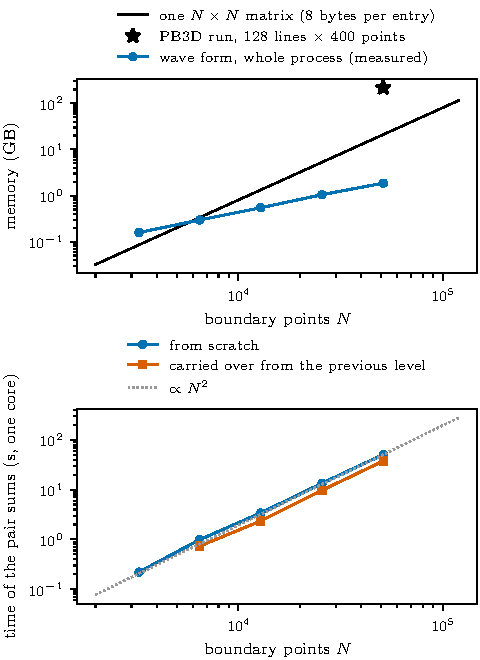
\includegraphics[width=\textwidth]{fig_cost.pdf}
\caption{Cost of the wave form on 64 lines, 51 to 801 points per line, one process on a laptop. (a) Peak memory of the whole process, against one $N\times N$ matrix of doubles and the 220~GB of PB3D's run with 128 lines $\times$ 400 points. (b) Time of the pair sums from scratch and carried over from the previous level.}
\label{fig:cost}
\end{figure*}

\subsection{Single waves as data}
In PB3D the normal data are not exact harmonics but the modes of the plasma window, each a single wave.
With $q = e^{\imath(n\varphi - m\theta)}$ for $m = 6$, 11 and 15 as data, on 64 lines $\times$ 201 points and with 50 waves ($m = -14$ to 35), the potential stays concentrated on the wave of the data.
Relative to that wave, the neighbours $m\pm1$ carry 0.1 to 6\,\%, the waves $m\pm2$ 0.2 to 1.1\,\%, the waves $m\pm3$ 0.03 to 0.12\,\%, and all waves further away less than $2.5\times10^{-4}$, a floor that no longer falls with the distance from the data wave.
For data of this kind, three or four sidebands on each side of the plasma window would reach that floor.
This holds for waves in the geometric angle on a circular torus; for PB3D's straight-field-line angle and for shaped boundaries it is not tested.

\subsection{Accuracy against the point-value form}
Figs.~\ref{fig:accuracy}(b) and (c) compare the two forms on the same grids.
The energy errors coincide to the digits shown wherever both were run: on 64 lines $\times$ 201 points they are $3.1\times10^{-3}$, $1.4\times10^{-2}$ and $3.3\times10^{-2}$ for $m = 6$, 11 and 15 in both forms.
The errors of $\Phi$ itself are slightly smaller with waves: $3.2\times10^{-3}$, $1.4\times10^{-2}$ and $3.4\times10^{-2}$, against $3.6\times10^{-3}$, $1.5\times10^{-2}$ and $3.5\times10^{-2}$.

The two forms were also compared with each other directly.
On 64 lines $\times$ 201 points with $k = 12$, their energies differ by $4.2\times10^{-7}$, $2.1\times10^{-6}$ and $4.0\times10^{-6}$ for $m = 6$, 11 and 15, about a thousand times less than either differs from the exact energy, while their potentials differ at the points by $1.6\times10^{-3}$, $4.4\times10^{-3}$ and $7.7\times10^{-3}$, less than either form's own error in $\Phi$.
The residual of the wave form is orthogonal to the waves, and the data $q$ lie almost within their span, so the residual hardly reaches the energy.
With $k = 6$ the energies for $m = 15$ differ by 4.7\,\%, so the direct difference also shows when the waves are too few.
On 64 $\times$ 101 with $k = 12$ the energy differences are $9\times10^{-7}$ to $3\times10^{-5}$.

With this plain rule, the error is set by the number of field lines, not by the points along them.
From 201 to 801 points per line the errors change by less than 8\,\% (Fig.~\ref{fig:accuracy}(b)), while each doubling of the lines from 16 to 128 reduces them by a factor 4 to 12 (Fig.~\ref{fig:accuracy}(c)).
On 16 lines the errors for $m = 11$ and 15 exceed 100\,\%, in both forms.
The kernel between two neighbouring lines is summed with one point per line in the direction across the lines; PB3D's near-field rule of 31 October 2026 treats this along the lines, and the prototype does not include it.

\subsection{Carry-over, memory and time}
From 51 to 801 points per line, every level was computed twice: from scratch, and carried over from the previous level with Eq.~\eqref{eq:carry}.
The largest relative difference of $\mtx{A}^\text{pair}$, $\vec{b}^\text{pair}$ and $S_i$ between the two is $4.7\times10^{-16}$ to $8.9\times10^{-16}$, i.e.\ rounding.

Fig.~\ref{fig:cost}(a) gives the peak memory of the whole Python process for the wave form, measured separately for each grid on 64 lines.
It grows about in proportion to $N$, by a factor 1.8 to 1.9 per doubling, from 0.16~GB at $N = 3\,264$ to 1.9~GB at $N = 51\,264$.
At the largest grid the parts were measured separately: the evaluation of the exact harmonics for the test data alone peaks at 0.69~GB, because Laplace's integral is taken on 512 points for all $N$ boundary points at once; the pair sums then add 1.2~GB with blocks of 256 rows of kernel values and their temporaries, and 0.38~GB with blocks of 64 rows, for 11\,\% more time.
The three numbers add up as if the data's memory stayed allocated, so the method itself needs the block plus about 0.1~GB of per-point arrays, and the 1.9~GB of Table~\ref{tab:criteria} includes 0.69~GB that belongs to the test data.
One $N\times N$ matrix of doubles at the largest grid takes 21~GB, and PB3D's run of the same size was given 220~GB.

Fig.~\ref{fig:cost}(b) gives the time of the pair sums; the process used 98 to 101\,\% of one core.
It grows with $N^2$, as the number of pairs does; carrying a level over takes 0.69 to 0.74 of the time from scratch, close to the three quarters of the pairs that remain to be computed.

\section{What is not tested}\label{sec:open}
\begin{itemize}
\item The near-field rule. PB3D integrates the kernels along the line within four intervals of the singular point, on a cubic interpolant. These near pairs change when points are added, so they would need their own sums, rebuilt at every level; the far pairs carry over as above.
\item A stellarator. On a non-axisymmetric boundary the potential also contains the toroidal mode numbers $n\pm N_\text{fp}$, $n\pm2N_\text{fp}$, \ldots, with $N_\text{fp}$ the number of field periods, so the set of waves grows. By how much is not known; W7-X is the obvious test, with the exact potentials of PB3D's \texttt{check\_vac}.
\item PB3D's own data. In PB3D the normal data are the modes of the plasma window (\texttt{EP} in \texttt{calc\_vac\_res}), so $\vec{b}$ becomes an $M'\times M$ matrix, carried over in the same way.
\item Flux coordinates. The waves here use the geometric poloidal angle; in PB3D they would use the straight-field-line angle of the plasma modes.
\item Fortran, MPI and the time per level in PB3D.
\end{itemize}

\section{Conclusion}\label{sec:conclusion}
With the potential at the boundary points as unknowns, the field-line vacuum of PB3D needs all points at every Richardson level, as Ref.~\onlinecite{Weyens2019vacuum} states, and its memory grows fourfold per level.
With the amplitudes of a few dozen waves as unknowns, the same rows of $\mtx{H}$ and $\mtx{G}$ give a small system whose entries are sums over pairs of points.
These sums carry over from one level to the next as one quarter of the old sums plus the pairs with a new point, as the plasma integrals do with one half, and no $N\times N$ matrix is stored.
On a circular torus with exact toroidal harmonics, the wave form is as accurate as the point-value form on the same rows and runs 51\,264 boundary points in 1.9~GB.
It needs 34 waves for a window of 10 modes when the data are the exact harmonics, which are spread over many waves in the geometric angle; with single waves as data, as the plasma modes of PB3D are, the potential stays on the wave of the data and three or four sidebands on each side would do.
This is an exploration; whether the wave form enters PB3D is not decided.
The next checks would be the number of waves on a W7-X boundary, and the wave form together with the near-field rule.

\begin{acknowledgments}
The idea to make the vacuum keep integrals rather than points, as the plasma does, is Toon Weyens's.
\end{acknowledgments}

\begin{thebibliography}{6}

\bibitem{Weyens2017PB3D}
T.~Weyens, R.~S{\'{a}}nchez, G.~Huijsmans, A.~Loarte, and L.~Garc{\'{i}}a,
``PB3D: A new code for edge 3-D ideal linear peeling-ballooning stability,''
J.\ Comput.\ Phys.\ \textbf{330}, 997--1009 (2017).

\bibitem{Weyens2019vacuum}
T.~Weyens, ``Expressions for perturbed vacuum potential energy for 3D linear MHD stability,'' manuscript (21 March 2019).

\bibitem{Sauter2011BEM}
S.~A.~Sauter and C.~Schwab, \emph{Boundary Element Methods} (Springer, Berlin, 2011).

\bibitem{Merkel1986}
P.~Merkel, ``An integral equation technique for the exterior and interior Neumann problem in toroidal regions,'' J.\ Comput.\ Phys.\ \textbf{66}, 83--98 (1986).

\bibitem{Merkel1996}
P.~Merkel, C.~N{\"u}hrenberg, and W.~A.~Cooper, ``Free-boundary ideal MHD modes in W7-AS,'' CRPP Lausanne report LRP 555/96, 51--58 (1996).

\bibitem{DLMF14}
\emph{NIST Digital Library of Mathematical Functions}, chapter~14, Legendre and related functions, \url{https://dlmf.nist.gov/14}.

\end{thebibliography}

\end{document}
